% Multi-seed defense effectiveness across attacks at 2C calibration (3 seeds).
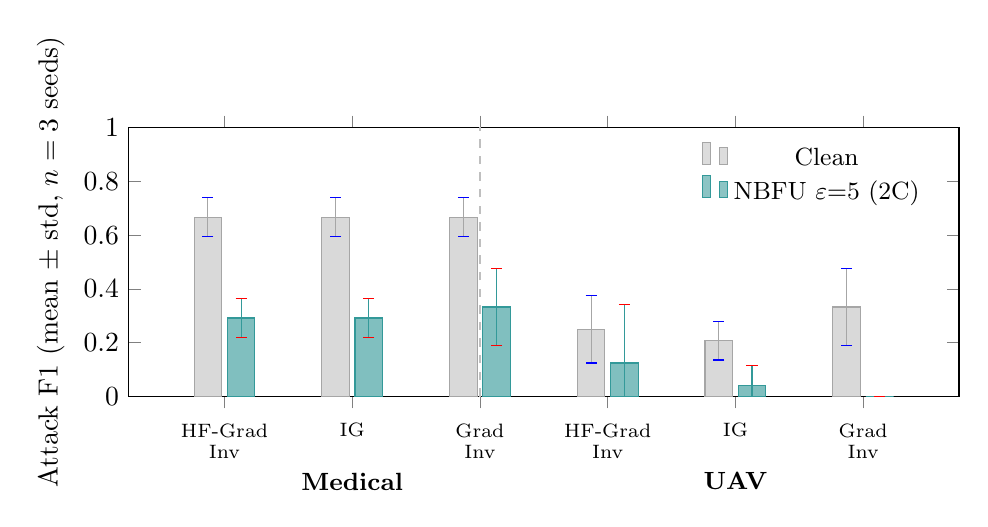
\begin{tikzpicture}
\begin{axis}[
    width=\columnwidth,
    height=5cm,
    ybar=2pt,
    bar width=10pt,
    enlarge x limits=0.15,
    ylabel={Attack F1 (mean $\pm$ std, $n=3$ seeds)},
    symbolic x coords={HF-GradInv, IG, GradInv, HF-GradInv*, IG*, GradInv*},
    xtick={HF-GradInv, IG, GradInv, HF-GradInv*, IG*, GradInv*},
    xticklabels={\shortstack{HF-Grad\\Inv}, IG, \shortstack{Grad\\Inv}, \shortstack{HF-Grad\\Inv}, IG, \shortstack{Grad\\Inv}},
    xticklabel style={font=\scriptsize, align=center, yshift=-2pt},
    extra x ticks={IG, IG*},
    extra x tick labels={Medical, UAV},
    extra x tick style={
        major tick length=0pt,
        xticklabel style={yshift=-22pt, font=\small\bfseries}
    },
    ymin=0, ymax=1.0,
    legend pos=north east,
    legend style={font=\small, draw=none, fill=white, fill opacity=0.9, text opacity=1},
    error bars/y dir=both,
    error bars/y explicit,
]
\addplot+[fill=gray!30, draw=gray!70] coordinates {
    (HF-GradInv, 0.667) +- (0,0.072)
    (IG, 0.667) +- (0,0.072)
    (GradInv, 0.667) +- (0,0.072)
    (HF-GradInv*, 0.250) +- (0,0.125)
    (IG*, 0.208) +- (0,0.072)
    (GradInv*, 0.333) +- (0,0.144)
};
\addlegendentry{Clean}

\addplot+[fill=teal!50, draw=teal!80] coordinates {
    (HF-GradInv, 0.292) +- (0,0.072)
    (IG, 0.292) +- (0,0.072)
    (GradInv, 0.333) +- (0,0.144)
    (HF-GradInv*, 0.125) +- (0,0.217)
    (IG*, 0.042) +- (0,0.072)
    (GradInv*, 0.000) +- (0,0.000)
};
\addlegendentry{NBFU $\varepsilon{=}5$ (2C)}

\draw[gray!50, dashed] (axis cs:GradInv,0) -- (axis cs:GradInv,1.0);
\end{axis}
\end{tikzpicture}
